\documentclass[conference]{IEEEtran}
\IEEEoverridecommandlockouts
\usepackage{cite}
\usepackage{amsmath,amssymb,amsfonts}
\usepackage{graphicx}
\usepackage{textcomp}
\usepackage{xcolor}
\usepackage{booktabs}
\usepackage{multirow}
\usepackage{url}
\usepackage{tikz}
\usetikzlibrary{arrows.meta,fit}
% Public repository with code, prompts, generated solvers and analysis scripts.
\newcommand{\repourl}{\url{https://github.com/VARUN3WARE/finreason-cup-2026}}

\begin{document}
\bstctlcite{IEEEexample:BSTcontrol}

\title{HumanSlop at FinReason Cup 2026 Tasks 1 and 3: Verified Program Synthesis for Exact Financial Reasoning and Executable Rule Semantics for XBRL Audit Verification}

\author{
\IEEEauthorblockN{Varun Rao}
\IEEEauthorblockA{\textit{Independent Researcher}\\
Kanpur, India\\
varunrao.gd@gmail.com}
\and
\IEEEauthorblockN{Galaba Vamsi}
\IEEEauthorblockA{\textit{Independent Researcher}\\
Bengaluru, India\\
galabavamsi12@gmail.com}
}

\maketitle

\begin{abstract}
FinReason Cup 2026 Task 1 asks systems to solve multi-step financial word problems and to report not only a final
answer but also the values of published intermediate reasoning checkpoints, scored by exact match---often against
exact rational numbers. We treat this setting as \emph{program synthesis with verification}
rather than as free-form chain-of-thought generation. Our system has two tiers.
For the 290 problem structures observed in training, LLM coding agents induce one executable solver per structure,
using exact rational arithmetic, and a solver is admitted (\emph{verified}) only after it reproduces all 11 labeled
instances of its structure. For the never-seen structures in the test set no labels exist, so nothing can be verified
in that sense; there we use a gold-free cross-checking protocol. Four independent
``lenses'' (literal transcription, finance-model-first, ambiguity hunting, and hand-solve-first), run on
three models from one provider, each synthesize a solver for a cluster of structurally identical questions, and
field-level disagreements go to blind adjudicators who must justify every ruling from the question
text. Three no-execution reasoning passes, an adversarial red team and blind reviewers then cross-examine every
decision without labels, a six-juror blind jury settles the contested fields, and metamorphic perturbation
serves as a diagnostic. On the development leaderboard the
system scores \textbf{1.000} on both final answers and reasoning steps (best organizer baseline 0.984/0.990); on the
official test set it ranks 11th of 27 teams (923 of 928 final answers correct, hidden-structure FAC 0.998).
A single gold-free agent per topic reproduces all 3{,}190 labeled training and
development instances. On the 116 hidden test structures, 112 were unanimous across the four lenses,
and the final programs agree with independent no-execution reasoning on 99.6\% (Opus), 99.5\% (Sonnet) and 98.8\% (Fable) of fields.
A stage-wise ablation shows that the literal lens alone already yields every final answer we submitted: the later
stages changed six of 456 checkpoint values and account for most of the cost, so they bought assurance rather than accuracy.
The residual disputes all concern interpretation, and they cluster by model. For Task~3 (XBRL audit
verification), we re-implement the three Data Quality Committee rules behind the cases from their official XULE source
and infer which rule fired from each rule's scope. This lifts development accuracy from the organizer baseline's
33.09\% to 98.38\%, with all 464 statement-calculation (DQC\_0126) cases correct, and scores 96.03\% on the official
test set (11th of 23 teams).
\end{abstract}

\begin{IEEEkeywords}
financial reasoning, program synthesis, verification, large language models, LLM agents, exact arithmetic
\end{IEEEkeywords}

%=====================================================================
\section{Introduction}
%=====================================================================
Financial reasoning is a domain in which a plausible answer is not good enough: a single misplaced rounding step, an
inverted sign, or a percentage read as a ratio produces a number that is wrong in a way that matters. The FinReason
Cup 2026~\cite{finreason2026overview} Task 1, \emph{Verifiable Financial Chain Reasoning}~\cite{finreason2026task1overview},
operationalizes this concern by building on the symbolic FinChain benchmark~\cite{xie-etal-2026-finchain}: each problem
is generated from a template, and a system must return a final answer together with the values of up to three
published intermediate ``checkpoints''. Both are scored by exact match. Many checkpoints must be reported as
\emph{exact} rationals (e.g.\ \texttt{636000/529}), so any floating-point or mentally rounded intermediate result is
simply wrong.

This scoring rule changes the design problem. Chain-of-thought prompting~\cite{wei2022cot} and self-consistency
voting~\cite{wang2023selfconsistency} improve the likelihood of a correct \emph{final} answer, but they give no
guarantee that intermediate values are exact, and they pay the full inference cost for every question. Program-aided
approaches~\cite{chen2023pot,gao2023pal} delegate arithmetic to
an interpreter and are therefore a better fit. We push this idea one step further: since every Task 1 question is an
instance of a reusable \emph{structure}, we synthesize one program per structure, not per question, and spend our
verification budget at the structure level, where it can be checked against several instances at once. Our own
no-execution baseline (Section~\ref{sec:exp-cot}) shows that a current frontier model can be exact on problems with
explicitly stated formulas. The case for programs here therefore rests on determinism, auditability, amortized
test-time cost and cross-instance checking, not on arithmetic alone.

\textbf{What ``verified'' means here.} We call a solver \emph{verified} only if it was admitted after reproducing every
labeled instance of its structure. That is possible for the 290 seen structures and for nothing else, and it is what
the title refers to. For hidden structures we speak of \emph{cross-checked} or \emph{decided} solvers. Agreement
between independently generated programs is evidence, not proof: Sections~\ref{sec:exp-triple}
and~\ref{sec:exp-official} report answers on which every check agreed and the official score still disagreed.

Our contributions are:
\begin{enumerate}
\item A structural analysis of the Task 1 data showing that every development and test question can be routed
deterministically either to one of 290 seen templates or to one of 116 unseen clusters of exactly three questions
(Section~\ref{sec:data}).
\item A \emph{verified program library}: one exact-arithmetic solver per seen structure, written by LLM coding agents and
admitted only after reproducing all labeled instances, plus an independent gold-free re-implementation used as an
$N$-version cross-check~\cite{avizienis1985nversion} (Section~\ref{sec:library}).
\item A \emph{gold-free multi-lens synthesis and adjudication} protocol for never-seen structures. It combines prompt
diversity, three models, behavioral comparison of programs~\cite{li2022alphacode,chen2023codet},
text-grounded adjudication, cross-modal no-execution checks, an asymmetric red-team review, a model-balanced jury, and
metamorphic perturbation as a label-free diagnostic of latent disagreement
(Sections~\ref{sec:hidden}--\ref{sec:redteam}).
\item For Task~3, executable re-implementations of the three DQC rules behind the cases, taken from the official XULE
source, together with label-free routing by rule scope (Section~\ref{sec:task3}).
\item An empirical study covering development-leaderboard results, a blindness-audited zero-shot ablation, a
no-execution chain-of-thought baseline, agreement statistics on the hidden structures, and a stage-wise ablation with
token costs that shows which stages changed any output (Section~\ref{sec:exp}).
\end{enumerate}

%=====================================================================
\section{Related Work}
%=====================================================================
\textbf{Numerical reasoning in finance.} FinQA~\cite{chen2021finqa}, TAT-QA~\cite{zhu2021tatqa} and
ConvFinQA~\cite{chen2022convfinqa} established numerical question answering over financial reports, and typically
score only the final answer. FinChain~\cite{xie-etal-2026-finchain} introduced symbolic, template-generated problems with
verifiable intermediate steps; FinReason Task 1 adopts this view and adds exact-rational checkpoint scoring as well as a
held-out set of unseen structures.

\textbf{Reasoning with programs.} Program-of-Thoughts~\cite{chen2023pot} and PAL~\cite{gao2023pal} have the model write
code and leave execution to an interpreter. Tool-making work~\cite{cai2024toolmakers} and library learning~\cite{ellis2021dreamcoder}
reuse synthesized functions across tasks, which matches our per-structure solvers. Agentic loops that interleave reasoning
with execution~\cite{yao2023react} let a model test its own code before committing to it.

\textbf{Selection and verification.} Self-consistency~\cite{wang2023selfconsistency}, trained
verifiers~\cite{cobbe2021verifiers,lightman2024verify}, execution-based clustering of candidate
programs~\cite{li2022alphacode,chen2023codet} and multi-agent debate~\cite{du2024debate} all exploit redundancy to choose
among candidates. Our hidden-structure protocol is closest to $N$-version programming~\cite{avizienis1985nversion}: we
deliberately diversify how independent versions are produced, then compare their \emph{behavior} field by field.

%=====================================================================
\section{Task and Data Analysis}\label{sec:data}
%=====================================================================
\subsection{Format and scoring}
Each question carries an \texttt{answer\_spec} (decimal with half-up rounding to a given number of places, an exact
rational, or an enum vocabulary) and a \texttt{trace\_spec} listing 0--3 checkpoint slots, each with its own
\texttt{result\_spec}. A prediction gives a final value and one value per slot. The official
scorer~\cite{finreason2026task1overview} compares decimal values after half-up rounding to the specified number of
places, compares exact values by rational equality, and compares enums by string. Scores are aggregated
hierarchically (template $\rightarrow$ difficulty cell $\rightarrow$ topic $\rightarrow$ domain), and the official test score
averages a \emph{seen} stratum (580 questions) and a \emph{hidden} stratum (348 questions) with equal weight. Ranking uses
the tuple (combined final-answer score, hidden final-answer score, combined checkpoint score), so performance on unseen
structures both carries half the weight and decides ties.

\subsection{Structural routing}
We define the \emph{signature} of a question as its answer specification together with the ordered list of slot ids,
descriptions and result specifications. The 3{,}190 labeled training and development questions have 267 distinct
signatures. Every template has exactly one, and 7 signatures are shared by more than one template (30 templates in all:
one signature covers 16 templates, one covers 4, and five cover 2 each). For those we mask every number in the question
body (integers, decimals and fractions, with an optional sign, become \texttt{\#}) and choose the candidate template
whose labeled instances contain the most similar masked text under the Ratcliff--Obershelp ratio of Python's
\texttt{difflib}. In practice no fuzzy matching was needed: all 120 unlabeled questions with a shared signature have a
masked text identical to that of a labeled instance.

Applying this router to the unlabeled splits yields a clean partition (Table~\ref{tab:splits}). All 580
development-leaderboard questions map to seen templates, two per template. Of the 928 test questions, 580 map to seen
templates (two per template), and the remaining 348 carry signatures that occur nowhere in the labeled data: 116
distinct signatures with exactly three questions each. A question is treated as hidden exactly when its signature is
unseen, so no similarity threshold is involved. The partition matches the official stratum sizes. The hidden structures
differ visibly from the seen ones: they
use longer prose without explicit formulas, numeric fields rounded to 2, 4, 6 or 8 places rather than exact
rationals, and more enum decisions (28 of 116 clusters), including tie-break rules (30 clusters) and solve-for
conditions (14 clusters).

\begin{table}[t]
\centering
\caption{Task 1 splits after structural routing.}
\label{tab:splits}
\begin{tabular}{lrrr}
\toprule
Split & Questions & Structures & Per structure \\
\midrule
Train (labeled) & 2{,}900 & 290 seen & 10 \\
Dev (labeled) & 290 & 290 seen & 1 \\
Dev leaderboard & 580 & 290 seen & 2 \\
Test -- seen & 580 & 290 seen & 2 \\
Test -- hidden & 348 & 116 unseen & 3 \\
\bottomrule
\end{tabular}
\end{table}

%=====================================================================
\section{System}
%=====================================================================
\begin{figure*}[t]
\centering
% Architecture of the Task 1 pipeline (Fig. 1). Included from main.tex with \input{fig_pipeline}.
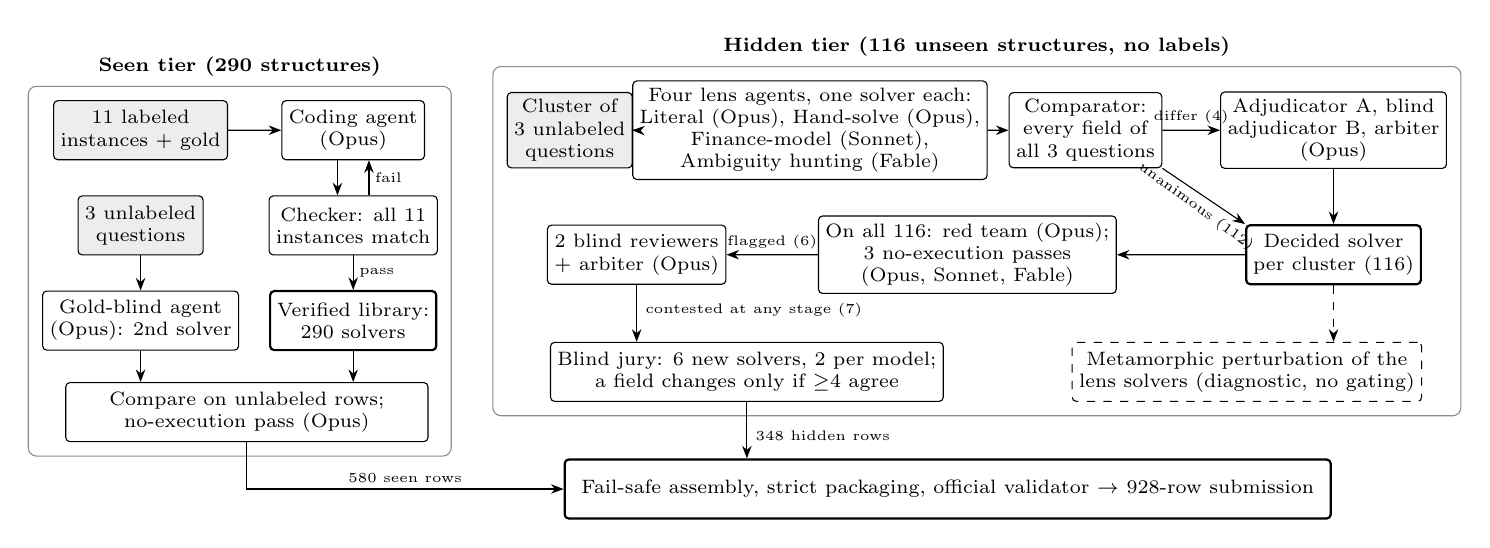
\begin{tikzpicture}[yscale=0.93,
  font=\scriptsize, >={Stealth[length=1.6mm]},
  box/.style={draw, rounded corners=1.5pt, align=center, inner sep=2.5pt, minimum height=7.5mm, fill=white},
  io/.style={box, fill=black!7},
  key/.style={box, line width=0.8pt},
  diag/.style={box, dashed},
  lab/.style={font=\tiny, inner sep=1pt},
  panel/.style={draw=black!45, rounded corners=3pt, inner sep=5pt},
]
% ---------------- seen tier ----------------
\node[io]  (s-in)    at (1.05,4.15) {11 labeled\\instances + gold};
\node[box] (s-agent) at (3.75,4.15) {Coding agent\\(Opus)};
\node[box] (s-check) at (3.75,2.85) {Checker: all 11\\instances match};
\node[key] (s-lib)   at (3.75,1.55) {Verified library:\\290 solvers};
\node[io]  (s-un)    at (1.05,2.85) {3 unlabeled\\questions};
\node[box] (s-blind) at (1.05,1.55) {Gold-blind agent\\(Opus): 2nd solver};
\node[box, minimum width=4.6cm] (s-cmp) at (2.4,0.3) {Compare on unlabeled rows;\\no-execution pass (Opus)};
\draw[->] (s-in) -- (s-agent);
\draw[->] ([xshift=-2mm]s-agent.south) -- ([xshift=-2mm]s-check.north);
\draw[->] ([xshift=2mm]s-check.north) -- node[lab,right=1pt]{fail} ([xshift=2mm]s-agent.south);
\draw[->] (s-check) -- node[lab,right=1pt]{pass} (s-lib);
\draw[->] (s-un) -- (s-blind);
\draw[->] (s-blind.south) -- (s-blind.south |- s-cmp.north);
\draw[->] (s-lib.south) -- (s-lib.south |- s-cmp.north);
\node[panel, fit=(s-in)(s-agent)(s-lib)(s-blind)(s-cmp),
      label={[font=\scriptsize\bfseries]above:Seen tier (290 structures)}] (seen) {};
% ---------------- hidden tier ----------------
\node[io]  (h-in)   at (6.5,4.15) {Cluster of\\3 unlabeled\\questions};
\node[box] (h-lens) at (9.55,4.15) {Four lens agents, one solver each:\\Literal (Opus), Hand-solve (Opus),\\Finance-model (Sonnet),\\Ambiguity hunting (Fable)};
\node[box] (h-cmp)  at (13.05,4.15) {Comparator:\\every field of\\all 3 questions};
\node[box] (h-adj)  at (16.2,4.15) {Adjudicator A, blind\\adjudicator B, arbiter\\(Opus)};
\node[key] (h-dec)  at (16.2,2.45) {Decided solver\\per cluster (116)};
\node[box] (h-chk)  at (11.55,2.45) {On all 116: red team (Opus);\\3 no-execution passes\\(Opus, Sonnet, Fable)};
\node[box] (h-rev)  at (7.35,2.45) {2 blind reviewers\\+ arbiter (Opus)};
\node[box] (h-jury) at (8.75,0.85) {Blind jury: 6 new solvers, 2 per model;\\a field changes only if $\geq$4 agree};
\node[diag] (h-meta) at (15.1,0.85) {Metamorphic perturbation of the\\lens solvers (diagnostic, no gating)};
\draw[->] (h-in) -- (h-lens);
\draw[->] (h-lens) -- (h-cmp);
\draw[->] (h-cmp) -- node[lab,above=1pt]{differ (4)} (h-adj);
\draw[->] (h-adj) -- (h-dec);
\draw[->] (h-cmp.south east) -- node[lab,sloped,below=1pt]{unanimous (112)} (h-dec.north west);
\draw[->] (h-dec) -- (h-chk);
\draw[->] (h-chk) -- node[lab,above=1pt]{flagged (6)} (h-rev);
\draw[->] (h-rev.south) -- node[lab,right=2pt,pos=0.45]{contested at any stage (7)} (h-rev.south |- h-jury.north);
\draw[->,dashed] (h-dec.south) -- (h-dec.south |- h-meta.north);
\node[panel, fit=(h-in)(h-lens)(h-adj)(h-dec)(h-jury)(h-meta),
      label={[font=\scriptsize\bfseries]above:Hidden tier (116 unseen structures, no labels)}] (hid) {};
% ---------------- assembly ----------------
\node[key, inner xsep=6pt, minimum width=9.6cm] (out) at (11.3,-0.75)
     {Fail-safe assembly, strict packaging, official validator $\rightarrow$ 928-row submission};
\draw[->] (s-cmp.south) |- node[lab,pos=0.75,above=1pt]{580 seen rows} (out.west);
\draw[->] (h-jury.south) -- node[lab,right=2pt,pos=0.6]{348 hidden rows} (h-jury.south |- out.north);
\end{tikzpicture}
\caption{The Task 1 pipeline. The seen tier is verified against labels; the hidden tier is cross-checked without
them. Numbers in parentheses on arrows are cluster counts on the hidden test set. Opus, Sonnet and Fable denote Claude
Opus 5.5, Sonnet 5.5 and Fable 5.1.}
\label{fig:pipeline}
\end{figure*}
Fig.~\ref{fig:pipeline} gives an overview of the two tiers.

\subsection{Exact execution substrate}
Every solver is a Python module that exposes \texttt{solve(text, question)} and returns a final value and one value per
slot as Python \texttt{Fraction}s (or an enum token). Floats are rejected at render time. Integer powers stay exact.
When non-integer powers, roots, logarithms or exponentials are genuinely needed, helpers evaluate them with 80-digit
decimal precision and convert the result back to a \texttt{Fraction}, which makes half-up rounding at the required
precision safe. The conversion is direct, with no rational reconstruction, so these helpers serve decimal-rounded
fields only; an exact tie reached through an irrational intermediate step would need symbolic simplification, which
we do not attempt. A shared renderer turns each value into the canonical string required by its
specification: a finite
decimal when the rational terminates in base 10, otherwise an irreducible \texttt{p/q}; half-up values are rounded
with integer arithmetic, and ties go away from zero ($-1.5 \rightarrow -2$), as in the official scorer. Solvers always
return \emph{unrounded} quantities, so ``independently rounded'' checkpoints can
never leak into downstream computation unless the problem text explicitly says they should.

\subsection{Verified program library for seen structures}\label{sec:library}
For each of the 58 topics (5 templates each), a coding agent (Claude Opus 5.5) is given a command that prints all 11
labeled instances
of a template together with their gold values. It writes one solver module per template and iterates until a checker
confirms that (i) all 11 labeled instances match on the final answer and on every slot, and (ii) the solver runs
without error and produces schema-valid output on the template's unlabeled leaderboard and test questions. Agents were
told to anchor number extraction on surrounding words rather than on positions, and to implement every stated
conditional rule (strict versus non-strict thresholds, ties, sign preservation) even for branches that no labeled
example exercises. At inference time the template id returned by the router selects the solver.

\textbf{$N$-version cross-check.} After the library was built, an independent agent for each topic wrote a
\emph{second} solver for each template while blind to gold values, to the library and to the checker
(Section~\ref{sec:exp-zs}). It saw only three unlabeled questions per template. Disagreement between the two versions
on any unlabeled row flags a robustness problem. No such disagreement occurred (Section~\ref{sec:exp-triple}), so
the pipeline never had to resolve one.

\subsection{Gold-free multi-lens synthesis for hidden structures}\label{sec:hidden}
For a hidden cluster of three questions, four agents independently write a solver. Each agent is assigned a different
\emph{lens}:
\begin{itemize}
\item \textbf{Literal} (Claude Opus 5.5): transcribe the text sentence by sentence into variables and rules.
\item \textbf{Finance-model-first} (Claude Sonnet 5.5): state the economic model first, then implement it, recording every
place where the text overrides convention.
\item \textbf{Ambiguity hunting} (Claude Fable 5.1): enumerate every point on which two analysts could disagree, and resolve
each one with textual evidence before coding.
\item \textbf{Hand-solve-first} (Claude Opus 5.5): solve one instance by hand with exact fractions, then write a solver that
must reproduce that hand solution.
\end{itemize}
The three models are tiers of one provider's model line, not independent model families (their API identifiers
are \path{claude-opus-5-5}, \path{claude-sonnet-5-5} and \path{claude-fable-5-1}).
Each agent is told not to open or list any other agent's files; this isolation rests on instructions, not on a
filesystem sandbox. A deterministic comparator executes all versions on
all three questions and compares every rendered field (final answer and each slot). If all versions agree on every field
of every question, the cluster is accepted and the literal-lens solver is kept as its solver. Otherwise adjudicator~A
reads the question, every version and the
field-level disagreement table, decides each disputed field by quoting the words of the question that settle it
(majority counts as evidence, not proof), and writes a corrected solver. A second, independent adjudicator~B, who is
told not to read A's work, does the same. If A and B produce identical outputs, A is accepted. Otherwise an arbiter
reads both
rationales and writes the final solver. If B cannot run, A's ruling stands provisionally and the cluster is sent to
blind review (Section~\ref{sec:redteam}). Adjudicators and arbiters run on Opus.

Because the three questions in a cluster share one structure but differ in numbers, and sometimes in which branch of a
condition applies, a solver has to be correct as a \emph{program}, not just on a single answer. That gives each
version a free consistency check across instances.

\subsection{Cross-modal checks and red-team review}\label{sec:redteam}
When versions agree, that is weaker evidence than it looks if they share a model's blind spots. We therefore add two
further layers that do not write code and run on every hidden cluster.

\textbf{No-execution cross-checks.} Independent agents answer every hidden question by reasoning alone. They read the
question once, then may not use any tool, so the result is a different modality from the programs. We run three such
passes, one per model (Claude Opus 5.5, Sonnet 5.5 and Fable 5.1). Each field is compared with the program output using the
official matcher, and a cluster with a disagreement on any field is sent to review. The Opus and Fable passes ran
before the review stage. The Sonnet pass was added afterwards, together with the jury, so a cluster it flagged went
straight to the jury.

\textbf{Red-team review.} For every decided cluster, an adversarial reviewer is told that analysts can share blind
spots and is asked to find a reading under which the current outputs are \emph{wrong}. It checks, sentence by sentence,
which quantity each checkpoint denotes, units (percent, ratio, millions), strict versus non-strict comparisons,
tie-breaks, floors, whether rounding happens before reuse, and branch outcomes on every instance. It may raise a
challenge only if it can quote words the current solver violates, and it must implement its alternative as a solver.
A challenged cluster, or one with a cross-check disagreement, goes to two blind reviewers. If both uphold the current
solver, it stays. Otherwise an arbiter must find decisive textual evidence to overturn it, field by field. This
asymmetry is deliberate: four independent versions plus a cross-modal check are strong prior evidence, so a single
persuasive reviewer cannot flip a correct consensus. The red team, the reviewers and the review arbiter all run on Opus.

\textbf{Blind jury.} As a last step, every cluster that any stage had contested goes to a jury of six blind jurors, two
per model (Opus, Sonnet, Fable). Each juror sees only the question text, writes and runs its own exact solver,
and reports its outputs together with every point a careful analyst could read two ways. We fixed the decision rule
before looking at any verdict: a field changes only if at least four of the six jurors agree on one value that
differs from the current answer. A 3--3 split keeps the current answer. When the jury changes a field, the cluster's
solver is replaced by the program of a juror whose outputs equal the jury's decision on every field of all three
instances, so the assembly step always takes whole programs and never patches single fields.

\textbf{Metamorphic agreement.} As a gold-free diagnostic, we perturb each question's \emph{parameters} and check that
the independently written versions still agree. Two versions that coincide only on
the three real instances but encode different rules show up as latent disagreement. Number tokens are aligned by
position across the instances of a structure. A token with the same value in every instance is a structural constant
(a 365-day year, a fixed threshold) and is held fixed; the others are parameters. Each parameter is multiplied by a
factor drawn uniformly from $[0.85, 1.15]$. Integers stay integers of at least 1, and integers up to 12 are left
alone, because they are usually counts, periods or decimal places. Decimals keep their number of decimal places,
values strictly between 0 and 1 are capped at 0.99 so that rates remain rates, and in a rational $a/b$ only the
numerator moves. Signs are preserved. The new number replaces the old one in the question text, and the surrounding
words on which the solvers anchor stay untouched. We draw 10 seeded perturbations per question and run every version on
each. A trial counts as agreement when all versions return identical rendered outputs on every field and as
disagreement when they differ; it is excluded as not runnable when any version raises an exception, for instance on a
division by zero or a premise that no longer holds. This step produces and changes no answer. It ran after the
decisions were made and gates nothing.

\subsection{Fail-safe assembly}
Predictions are assembled deterministically. A hidden question takes the decided solver's output. If that solver fails
on the instance, it falls back to the other versions, ordered by the size of their agreement group, then to the
no-execution answer, and abstains only as a last resort. A strict packaging mode refuses to write the test file
unless all 580 seen rows come from the verified library and all 348 hidden rows come from decided solvers. A strict
rebuild reproduces the official submission exactly, so the fallback chain is a safeguard that this submission never
used. Every file
then goes through the official validator and packager. Rebuilding the development predictions reproduces, byte for
byte, the file that scored 1.000/1.000.

\subsection{Integrity protocol}
No human inspected or edited any test answer. Test-time inference is fully automated: the cluster partition, the
prompts and the decision rule were fixed before the pipeline ran on the test set. Agents could consult public
training and development data (for example, to confirm a phrasing convention), and the seen-structure library was on the
same filesystem, but no test labels exist anywhere.
We audited the transcripts of the gold-blind agents for any access to gold files, to the library or to the checker
(Section~\ref{sec:exp-zs}). Blindness throughout rests on instructions about which files not to open and, for the
gold-blind agents, on this audit; we did not use filesystem-level sandboxing. All workflow scripts with their prompts,
the generated solvers of every stage, the decision records and the scripts that compute the numbers in this paper are
available at \repourl.

%=====================================================================
\section{Experiments}\label{sec:exp}
%=====================================================================
\subsection{Seen structures}
The library contains 290 solvers. Every one of them reproduces all of its labeled instances: 3{,}190/3{,}190 final
answers and all 5{,}698 labeled slot values. On the official development leaderboard (580 unlabeled questions), our
first submission scored 1.000000 on final answers and 1.000000 on reasoning steps, the top score on the board, which
other teams share (Table~\ref{tab:dev}).

\begin{table}[t]
\centering
\caption{Development-leaderboard results (580 questions; official scorer).}
\label{tab:dev}
\begin{tabular}{lcc}
\toprule
System & Final answer & Reasoning steps \\
\midrule
Organizer rule-based reference & 0.021 & 0.012 \\
Organizer Lite baseline & 0.234 & 0.555 \\
Organizer Standard baseline & 0.981 & 0.988 \\
Organizer Advanced baseline & 0.984 & 0.990 \\
\midrule
HumanSlop (verified library) & \textbf{1.000} & \textbf{1.000} \\
\bottomrule
\end{tabular}
\end{table}

\subsection{Gold-free synthesis on seen structures}\label{sec:exp-zs}
To measure the gold-free protocol where labels do exist, we treated each of the 290 seen templates as if it were
unseen. A single agent (literal-style prompt, Claude Opus 5.5; one agent per topic, 58 in all) saw only three unlabeled
questions of the template and
wrote a solver. We then scored that solver on the template's 11 labeled instances. It was correct on all 290 templates
(3{,}190/3{,}190 final answers; 5{,}698/5{,}698 slots), and its outputs agreed exactly with the verified library on all
1{,}160 unlabeled leaderboard and test rows. A transcript audit found no access to gold, targets, manifests, the
library or the checker in any of the 58 agents. The two solver sets are textually similar (median normalized
similarity 0.92), which reflects how explicitly the seen templates state their formulas. Where the problems are
harder, implementations diverge (the least similar pair has similarity 0.46) while their behavior stays identical.
The agents' self-reported confidence was ``high'' for 280 templates and ``medium'' for 10, all of which were correct.

\subsection{Direct chain-of-thought baseline}\label{sec:exp-cot}
To separate the contribution of program execution from that of the underlying model, 29 agents (Claude Opus 5.5)
each answered 10 labeled development questions by reasoning alone. They could run one command to print their questions
and were forbidden any further tool use; the transcript audit confirms one read and one structured answer per agent.
Scored by the official development scorer, this baseline is also perfect: 290/290 final answers and 518/518 checkpoints,
including exact rationals such as \texttt{840892149/102910000}. Two conclusions follow. First, on seen structures with
explicitly stated formulas, a current frontier model no longer needs an interpreter in order to be exact. Second,
reasoning and programs reach the
answer in different ways, so we use the direct answer as an additional check on hidden structures
(Section~\ref{sec:exp-hidden}). The program library still has practical advantages: it is deterministic, auditable,
and essentially free at test time. Building it is a one-off cost, while direct reasoning costs about 4.8k
tokens per question every time it runs.

\subsection{Triple verification of the seen test stratum}\label{sec:exp-triple}
The 580 seen test questions are checked three ways, and all three agree on every field: (i)~the gold-verified
library; (ii)~the gold-blind re-implementations, which match on every row; and (iii)~a fresh no-execution pass in
which 58 agents each answered 10 seen test questions by reasoning alone, matching the library on 580/580 final answers
and 1{,}036/1{,}036 checkpoints. Under metamorphic perturbation of the varying parameters (10 trials per question), the
library and the gold-blind versions agree on 5{,}800/5{,}800 trials. In other words, they implement the same rules on
parameter values well beyond the observed instances, not just on the instances themselves. All three checks ran on one
model (Opus), so this unanimity is weaker evidence than it looks; the official results in
Section~\ref{sec:exp-official} bear that out.

\subsection{Why exact arithmetic matters}
We count fields whose exact value falls precisely on a half-up rounding tie, i.e.\ a value of the form
$k+\tfrac12$ units in the last kept place (Table~\ref{tab:ties}). Such ties are common: 3.8\% of labeled seen fields
and 8.1\% of hidden test fields. Several hidden parameters look chosen to produce them; for example, a ratio of
$0.500001$ halved gives exactly $0.2500005$ at six decimal places. Converting the exact value to a binary float and
formatting it to the required
number of places misrounds a sizeable share of them, and that is before counting any error accumulated
\emph{during} a floating-point computation, or the exact-rational checkpoints, which floats cannot represent at all.

\begin{table}[t]
\centering
\caption{Exact half-up ties among rounded fields, and fields a float pipeline would misround when formatting the exact
value. ``Fields'' counts fields with half-up decimal rounding only; exact-rational and enum fields are excluded.}
\label{tab:ties}
\begin{tabular}{lrrr}
\toprule
Set & Fields & Exact ties & Float misrounded \\
\midrule
Seen, labeled (train+dev) & 3{,}091 & 117 & 54 \\
Seen, leaderboard & 562 & 12 & 6 \\
Seen, test & 562 & 15 & 11 \\
Hidden, test & 720 & 58 & 22 \\
\bottomrule
\end{tabular}
\end{table}

\subsection{Hidden structures}\label{sec:exp-hidden}
No labels exist for the 348 hidden test questions, so we report the agreement structure of the gold-free protocol
(Table~\ref{tab:hidden}). The hidden set has 804 scored fields: 348 final answers, 84 of them enum decisions, and 456
checkpoints. The four lenses produced field-identical solvers for 112 of the 116 clusters on the first
pass. The remaining four went to adjudication. In h091 the full chain ran: the two blind adjudicators disagreed, and
the arbiter decided. In h031, h040 and h058, adjudicator~B could not run because the session hit a usage limit, so
A's ruling stood provisionally and all three clusters went to blind review. There, two further independent
reviewers and a red-team reviewer upheld A's ruling in every case. At this point, before the jury, the decided outputs
coincided with the literal lens on all 804 fields: it is the default solver of unanimous clusters, and adjudication
sided with it in all four disputes. Agreement with these pre-jury decisions was 99.9\% for the hand-solve lens (Opus),
99.1\% for the finance-model lens (Sonnet) and 98.6\% for the ambiguity-hunting lens (Fable). The jury then changed six
checkpoint values against both Opus lenses (see below). Measured against the submitted outputs, field agreement is
803/804 (99.9\%) for the finance-model lens, 799/804 (99.4\%) for the ambiguity-hunting lens, 798/804 (99.3\%) for the
literal lens and 797/804 (99.1\%) for the hand-solve lens.

Before the jury, the Opus and Fable no-execution passes agreed with the program outputs on 801/804 and 788/804
fields. The 16 Fable disagreements fall in five clusters (4 fields in h031 and 3 each in h027, h040, h091 and h105).
All 116 clusters were red-teamed, and the red team raised a concrete challenge in only one (h091). Six
clusters went to blind review. Four were the disputed clusters: in h031 and h040 the Fable pass also disagreed, and
in h091 both no-code passes did. The other two were unanimous clusters flagged only by the Fable pass (h027, h105).
In five of the six, both reviewers independently upheld the current solver. In h091 they split, and the arbiter kept
the current reading under the conservative rule. Review changed no answer. A third no-execution pass (Sonnet) then
agreed on 800/804 fields and flagged one further cluster (h012). The seven clusters contested at any stage went to
the six-juror jury (42 juror solvers). The jury confirmed every \emph{final} answer: 19 of the 21 finals were 6/6, one was 4--2 for the
current answer (h040, a zero floor), and one was a 3--3 split that keeps it (h031, operator semantics). It changed six
\emph{checkpoint} values: in h040 five jurors computed the ceiling-utilization checkpoint at
post-burn supply, and in h091 all six read attrition-case EBITDA as including the confirmed savings (102). The
solvers of jurors 2 and 1, respectively, match the jury's decision on every field and became the decided solvers of
these two clusters. Against the
submitted outputs, the no-execution passes agree on 801/804 (Opus, 99.6\%), 800/804 (Sonnet, 99.5\%) and 794/804
(Fable, 98.8\%) fields.

Under metamorphic perturbation we attempted 3{,}480 trials (348 questions, 10 each). Five of them, all in cluster
h010, made one version raise an exception and are excluded. On the remaining 3{,}475 runnable trials the four lens
solvers agreed in 3{,}365 (96.8\%). Latent disagreement appeared in 8 clusters: all four disputed clusters (in every
trial of h031, h040 and h091, and in 8 of 30 for h058), plus four clusters that are unanimous
on the real instances but whose versions encode different rules elsewhere (h001, h098, h102, h115; 12 trials in all).
Perturbation therefore recovers every
cluster that real-instance comparison flagged, without needing any labels. Because it was a diagnostic and not a
gate, the four latent-only clusters were not sent to review.

\begin{table}[t]
\centering
\caption{Gold-free protocol statistics on the 116 hidden test clusters (804 scored fields).}
\label{tab:hidden}
\begin{tabular}{lr}
\toprule
Statistic & Value \\
\midrule
Clusters unanimous across 4 lenses & 112 / 116 \\
Clusters adjudicated (full A, B, arbiter chain) & 4 (1) \\
Opus no-code agreement with final & 801 / 804 \\
Sonnet no-code agreement with final & 800 / 804 \\
Fable no-code agreement with final & 794 / 804 \\
Clusters red-teamed / sent to blind review & 116 / 6 \\
Answers changed by review & 0 \\
Clusters sent to the 6-juror jury & 7 \\
Final / checkpoint values changed by the jury & 0 / 6 \\
Metamorphic agreement (3{,}475 runnable trials) & 96.8\% \\
Exact half-up ties among rounded fields & 58 / 720 \\
\bottomrule
\end{tabular}
\end{table}

\subsection{Stage-wise ablation and cost}\label{sec:ablation}
Test labels are private, so we cannot score intermediate stages. What we can measure exactly is how much each stage
\emph{changed}. Table~\ref{tab:ablation} compares the outputs the pipeline would have produced had it stopped at a
given stage with the outputs we submitted.

\begin{table}[t]
\centering
\caption{Stage-wise ablation on the hidden stratum: number of final answers (of 348) and checkpoint values (of 456)
that differ from the submitted outputs, with cumulative hidden-stratum tokens. No labels are used.}
\label{tab:ablation}
\begin{tabular}{@{}lrrr@{}}
\toprule
Configuration & Tokens & Final & Chkpt. \\
\midrule
Literal lens only (Opus) & $\approx$8M & 0 & 6 \\
Hand-solve lens only (Opus) & $\approx$8M & 1 & 6 \\
Finance-model lens only (Sonnet) & $\approx$8M & 1 & 0 \\
Ambiguity-hunting lens only (Fable) & $\approx$8M & 2 & 3 \\
\midrule
Four lenses, per-field plurality$^\dagger$ & $\approx$28M & 0 & 6 \\
\quad + adjudication & $\approx$28M & 0 & 6 \\
\quad + no-execution passes, red team, review & $\approx$51M & 0 & 6 \\
\quad + six-juror jury (submitted) & $\approx$53M & 0 & 0 \\
\bottomrule
\end{tabular}

\smallskip
\raggedright\footnotesize $^\dagger$Ties go to the literal lens. A single lens is costed at 116 runs of the logged
average of 71k tokens per synthesis agent; synthesis includes an estimated 20M tokens for two unlogged runs.
\end{table}

The result is clear-cut. The literal lens alone already yields all 348 final answers that we submitted. Neither a
per-field plurality over the four lenses, nor adjudication, nor the red team and blind review changes a single field
relative to it. Only the jury does, and only in six checkpoint values (h040 and h091); whether those six changes are
corrections we cannot tell without labels. Each of the other three lenses, used alone, would differ from the
submission in at most two final answers. The seen stratum shows the same picture: the verified library alone is what we
submitted, and neither the gold-blind re-implementation nor the no-execution pass changed anything.

The later stages therefore bought assurance, not accuracy. They told us which 7 of the 116 clusters were contestable,
they quantified how far independent readings agree on the other 109, and they exposed the model correlation analysed in
Section~\ref{sec:disputes}. They did not move the final-answer score: every configuration with a zero in the ``Final''
column of Table~\ref{tab:ablation} would have received the same Combined and Hidden FAC as our submission.

\textbf{Cost.} The full pipeline used about 1{,}150 completed agent runs. Usage logs record 45.2M subagent tokens over
844 of them. Two synthesis runs
that a session restart interrupted did not report usage; at the logged per-agent average, they add roughly 20M more.
The hidden stratum accounts for about 53M of the resulting 65M tokens: synthesis about 28M (more than 460 lens-agent
runs, since some lenses were regenerated after interruptions), the three no-execution passes 15.9M (349 agents), the
red team 5.4M (114 agents), blind review 0.8M (16 agents), the adjudication of h091 0.2M and the jury 2.3M (42
agents). The seen stratum cost 12.3M: 8.2M for the library together with its gold-blind proxy (116 agents), 2.8M for
the no-execution pass over the seen test questions and 1.4M for the development baseline. A minimal pipeline, the
verified library plus the literal lens, would have cost roughly 16M tokens, about a quarter of the total, and would
have produced the same final answer for all 928 test questions. Test-time inference
on the seen stratum is free once the library exists, and the 928-row submission builds deterministically in about
20 seconds on a laptop CPU, most of it spent on structural routing.

\subsection{Would one instance per structure be enough?}\label{sec:oneinstance}
The protocol had three questions per unseen structure. Two measurements indicate how much of its ability to
\emph{detect} disputes would survive with one. First, we check on which instances each lens dispute is visible. In
h031, h040 and h091 the lenses disagree on every instance, so any single instance exposes the dispute. In h058 they
disagree only on the instance that violates the stated premise, so a single instance exposes it with probability one
third. The three disputed \emph{final} answers (one each in h031, h040 and h058) are each confined to one instance.
Second, we repeat the metamorphic diagnostic with one instance per structure. Without sibling instances, constants
cannot be told apart from parameters, so every number is perturbed (except integers up to 12, as before). Run
separately on each of the 348
questions, this flags all four disputed clusters: h031, h040 and h091 from every instance, and h058 from two of its
three. It also flags the four latent clusters found before and two more (h015, h090), which show disagreement only
once constants are perturbed. Perturbation thus replaces most of what extra instances contribute to
detection. What we did not measure is synthesis quality. The lens agents wrote their solvers with three instances in
view, and the ablation of Section~\ref{sec:exp-zs} also showed three. With a single instance, a branch that the
instance does not exercise is constrained by the text alone, and we would expect more latent disagreement of the h058
kind.

\subsection{Official test results}\label{sec:exp-official}
The official Task~1 test results (published 28 October under the frozen scorer) place us 11th of 27 teams, with
Combined FAC 0.995466, Hidden FAC 0.998016 and Combined checkpoint 0.992614; 923 of the 928 final answers are
correct. The implied seen-stratum FAC is 0.992916. The four leading teams answered 927 of 928 questions. All ten teams
above us scored a hidden FAC of at least 0.998, so places were decided almost entirely on the seen stratum.

Our hidden FAC is the smallest non-zero hidden loss on the board, and two other teams share it. That is consistent
with a single missed hidden question, which would put the other four misses on the seen stratum. One of them may be the
test question whose wording and frozen reference answer the organizers report as inconsistent: each of the four
leading teams also missed exactly one question while scoring 1.000 on the hidden stratum. That still leaves about three
seen test answers that were wrong although the verified library, the gold-blind re-implementation and the no-execution
pass agreed on every field (Section~\ref{sec:exp-triple}). We cannot identify them, because the test answers remain
private. Two explanations fit what we know. Test instances of seen structures may fall outside the parameter regions
that the 11 labeled instances cover (different branch outcomes or premise violations), where reproducing the labels
does not pin a solver down. And all three checks ran on one model, so a reading that this model prefers passes all of
them; Section~\ref{sec:disputes} documents the same effect on the hidden stratum. Either way, verification against
labeled instances covers the labeled region, and agreement among versions that share a model is weak evidence outside
it.

%=====================================================================
\section{Analysis of Hidden-Structure Disputes}\label{sec:disputes}
%=====================================================================
All four real-instance disputes, and every flag raised by the cross-checks, concern \emph{interpretation}. None
involves arithmetic, which the exact substrate makes uninteresting. They fall into three classes.

\textbf{Operator semantics.} In h031, ``reduce the base appetite by the downturn haircut'' was read multiplicatively,
$a(1-h)$, by three lenses and subtractively, $a-h$, by one (the Fable lens). The two readings give different
checkpoint values on all three instances, but the final answer is an enum decision, and it flips on only one of them.
Adjudication chose the multiplicative reading. It cited
the financial meaning of a haircut, the phrasing of proportional reductions elsewhere in the training data, and one
instance in which the multiplicative reading lands exactly on a half-up tie at six decimal places. The jury split
3--3 on this cluster, which keeps the current answer under our rule; it is the least settled final answer in the
hidden set.

\textbf{Floors and premise violations.} In h058 one instance violates the stated premise (the primary detection ratio
already exceeds the target), so the unclamped formula yields a negative ``minimum required'' detection ratio. Two
lenses floored it at zero and two did not; on the other two instances all four lenses agree. In h040 the Sonnet lens
floored a headroom quantity at zero that no sentence
floors, which changes the final answer of one instance. Adjudicators kept a floor only where the quantity is a share
that cannot be negative, and the jury confirmed both rulings (4--2 in h040).

\textbf{Checkpoint denotation.} The subtlest disputes concern \emph{which} intermediate quantity a checkpoint names.
In h040, separately from the floor above, the ceiling-utilization checkpoint can be computed from market
capitalization at the ``current'' (pre-burn) or at the post-burn supply. In h091 the checkpoint is ``recurring
EBITDA in the attrition state'', read as verified EBITDA minus the fall (91, 83 and 81 in the three instances) or as
valuation EBITDA including
confirmed run-rate savings (102 in every instance). In both clusters the final answers are identical under either
reading, and only three checkpoint values depend on the choice. Adjudication and review first kept the pre-burn
reading and the lower EBITDA values. The jury reversed both (5--1 and 6--0). In h091 all three no-execution passes also
give 102. In h040 the
Opus and Sonnet passes keep the pre-burn reading, which makes it the closest call in the hidden set. The h027 and h105 flags were also denotation questions (a ``one-period''
versus a cumulative growth multiple, and a surplus versus a total value). In both cases two blind reviewers and all
six jurors upheld the program reading.

\textbf{Model correlation.} Disagreement is not spread uniformly across models. On the denotation questions in h040
and h091 the four
lenses split two--two along model lines: both Opus lenses (literal and hand-solve) against the Sonnet and Fable
lenses. Adjudication, blind review and arbitration all ran on Opus, and each time they upheld the Opus reading. The
review rule protects the incumbent solver, so it carried that reading forward, and in the three clusters where
adjudicator~B could not run the incumbent was a single Opus ruling. The
model-balanced jury reversed both readings, and in h091 both Opus jurors joined the majority once they solved the
question
from scratch rather than ruling on existing code. The other disputes follow the same pattern. The zero floor in h040
appears in the Sonnet lens and in both Sonnet jurors, and in no Opus or Fable agent. The subtractive reading in h031
appears in the Fable lens, the Fable no-code pass and both Fable jurors, joined by one Sonnet juror. The Fable no-code
pass raised the only flags in h027 and h105; the Sonnet no-code pass raised the only flag in h012, which all six
jurors rejected. Interpretive tendencies thus travel with the model rather than with the prompt. A decision chain
that runs on one model can entrench that model's reading, so the final vote should be balanced across
models, and agreement within one model is weak evidence. All three of our models come from one provider. We did not
test models from other providers. Since even sibling models disagree in systematic ways, a jury that mixes providers
is the most direct way to reduce correlated error further, and it is the first change we would make.

%=====================================================================
\section{Task 3: Financial Audit Verification}\label{sec:task3}
%=====================================================================
\subsection{Task and data}
Task~3~\cite{finreason2026task3overview} builds on the FinMR task of FinAuditing~\cite{wang2026finauditing} and the
Herculean benchmark~\cite{peng2026herculeanagenticbenchmarkfinancial}. Each case ships one SEC filing (schema;
presentation, calculation, definition and label linkbases; instance document; taxonomy notes for the target concept)
and asks for the value \emph{reported} for a concept and period and the value \emph{implied} by the filing's own
relationships. Every case receives exactly one label, decided by the first check that fails: S (the answer is not a
valid two-field object), E (the extracted value is wrong), C (the extracted value is right and the calculated value is
not, with zero tolerance), otherwise A. ACC, SER, EER and CER denote the shares of cases labeled A, S, E and C. The
leaderboard returns a provisional score from a deterministic matcher and an official score from an LLM judge, which
also accepts numbers that are written differently but mean the same; we report official scores. Every case was
produced by one flagged XBRL US Data Quality Committee rule.
DQC\_0015 flags negative values of elements that must not be negative. DQC\_0117 cross-checks dimensional breakdowns in
statement tables. DQC\_0126 checks statement calculations on non-dimensional facts. The ranked phases do not reveal
which rule produced a case.

Two data facts shaped our approach. First, the public practice set is truncated: every XML section stops at about
32.8k characters (the Excel cell limit of 32{,}767 in the original build). As a result, the target fact is visible in only
207 of its 332 cases, whereas the development and test filings are complete. Second, each hidden-phase case ships
exactly one presentation role, but it includes every fact of the concepts that role presents.

\subsection{Method: executable rule semantics}
Rather than asking a model to audit, we re-implement the three DQC rules from their official XULE
source and from the rule documentation. The gold answers are transcribed rule messages, so
\emph{extracted} is the value the message reports and \emph{calculated} is the value it says the filing implies.
\begin{itemize}
\item \textbf{DQC\_0126.} Only presentation networks whose definition contains ``- Statement -'' count, minus the rule's
exclusion lists and minus statement tables (hypercubes). For these, the calculated value is the weighted sum $S$ of the
target's direct calculation children. Children must share the total's unit. Facts are chosen by the rule's
\texttt{fs\_decimals} preference, and the rule fires only if
$|\mathrm{round}_d(T)-\mathrm{round}_d(S)| > 10^{-d}(n{+}1)$. Here $T$ is the reported total, $n$ is the number of
children that have a fact, and $d$ is the statement's \texttt{fs\_decimals}: the most frequent XBRL \texttt{decimals}
attribute among the non-dimensional facts of the statement's parent concepts ($d=-6$ for values reported in
millions; the tolerance is zero when $d$ is infinite).
\item \textbf{DQC\_0117.} For each statement hypercube and each of the 11 listed axes, assertion 9574 compares the
non-dimensional total with the sum of the highest reported level of nested members, subject to the rule's subtotal,
notes and parenthetical gates and its tolerance $2\cdot 10^{-t}$, where $t$ is the smallest \texttt{decimals}
attribute among the facts compared, capped at 5. Assertion 10093 compares a member's value with its
second-axis breakdown under the same tolerance, and applies only when no 9574 message exists. When only a disclosure
role is shipped, we fall back to summing declared members, and then
all single-dimension members.
\item \textbf{DQC\_0015.} Every non-nil negative fact of an element on the official list is a candidate unless it
carries an excluded member or axis. The calculated value is its magnitude.
\end{itemize}
Because the rule is hidden, the solver infers which rule fired. It tests each rule's \emph{scope}, not merely whether
some sum disagrees: 0015 when the element is on the list and a candidate exists, then 0117 on statement tables, then
0126 on qualifying statements. A case outside all three scopes goes through a fixed fallback chain: 0117 on any
shipped role, sums over the members declared for an axis, sums over all single-dimension members, a flagged negative
fact of an unlisted element, and finally the negated reported value. The fallbacks decide 4 of the 680 development
cases and 11 of the 680 test cases. On the development set, this routing reproduces the official per-rule
case counts exactly (162/54/464).

\subsection{Irreducible ambiguity and the selection heuristic}\label{sec:t3-ambiguity}
When a filing has several flagged negative facts for the same concept and period (for example, several dimension
members), the question does not say which one the case targets. The practice set keeps one case per flagged fact, but
the hidden phases keep one case per concept and period, and the emission order of the rule engine is not
reproducible. On the development set this affects 19 cases (about 2.8\%); a uniform guess would get about 6.5 of
them right. Because the leaderboard reports accuracy per rule, each development upload measures one selection policy on
exactly these cases. Document order scores 7/19, last-in-document 6, largest magnitude 4, alphabetical member order
5, raw-text order 8, and \emph{smallest magnitude} 12. No single ordering we tried (by value, text, context
identifier, document position, member or
axis name, or dimensionality) reproduces all six measurements, so the builder's choice is not a simple sort of the
facts the
filing contains. We adopted smallest magnitude (v7) because it scored best, and applied it only to listed elements,
where it was measured.

This is a choice among six policies on 19 cases, with no basis in the rule source, and it may overfit. With the
heuristic the development score on DQC\_0015 is 155/162 (95.68\%). Without it (document order, otherwise identical
code) it is 150/162 (92.59\%). Overall that is 98.38\% with the heuristic against 97.65\% without it; the second
figure follows from the per-rule scores, since that variant was not uploaded as a whole. On the test set
22 cases are ambiguous, a uniform guess would get about 4.9 of them right, and the heuristic changes 18 answers
relative to document order. Only each team's final test upload was scored, so no test score exists for the variant
without the heuristic; it can account for at most 3.2 points of test accuracy in either direction. Our test accuracy
on DQC\_0015 is 87.65\% (20 errors), against 7 errors on development. Either the
heuristic chose correctly in few of the ambiguous test cases, or the test set contains error types that
development did not; we cannot separate the two without labels. We therefore regard the heuristic as unvalidated
on test.

\subsection{Results}
\begin{table}[t]
\centering
\caption{Task 3 development leaderboard (680 cases, official LLM judge; ACC, EER and CER in percent).}
\label{tab:task3}
\setlength{\tabcolsep}{4.5pt}
\begin{tabular}{@{}lcccc@{}}
\toprule
System & ACC & EER & CER & Rank \\
\midrule
Organizer rule-based baseline & 33.09 & 3.97 & 62.79 & -- \\
v2: rule routing, no scope & 95.00 & 1.47 & 3.53 & 11 \\
v3: scope-based routing & 97.06 & 0.59 & 2.35 & 9 \\
v5: XULE-faithful 0117/0126 & 97.50 & 1.03 & 1.47 & 7 \\
v7: + 0117 no-total rule, 0015 min.\ magn. & 98.38 & 0.59 & 1.03 & 13$^\ast$ \\
\bottomrule
\end{tabular}

\smallskip
\raggedright\footnotesize $^\ast$Rank on 20 October. By then the board contained many near-duplicate team names with
identical scores, consistent with per-case probing. SER is 0.15\% for the baseline and 0 for all our versions.
\end{table}
Table~\ref{tab:task3} shows the progression. Routing by rule scope removed most of v2's misrouted negative-value
cases. Faithful re-implementations then fixed unit alignment, statement-table exclusion and the second-axis
assertion of 0117 (v5). Version v7 differs from v5 by six cases. One is a 0117 case gained by treating a missing
total as \emph{no} 9574 message, so that only 10093 can fire (v6, not uploaded on its own). Five are 0015 cases gained
by the selection heuristic of Section~\ref{sec:t3-ambiguity}. By rule, 0015 went from 12 errors (4 extraction, 8
calculation) to 7 (3 and 4), and 0117 from 5 errors (3 and 2) to 4 (1 and 3), which accounts for the three-case drop
in each of EER and CER. DQC\_0126 is at 464/464 from v5 on. On the test set v7 scores 96.03\% (extraction error
1.91\%, calculation
error 2.06\%), 11th of 23 teams; the joint winners reached 97.79\%. By rule, we score 100\% on 0126, 87.04\% on 0117
and 87.65\% on 0015. No team exceeded 91.98\% on 0015, which is consistent with the case-selection ambiguity limiting
every system. No step uses case identifiers or any external source of
DQC findings, which the competition rules forbid.

%=====================================================================
\section{Limitations}
%=====================================================================
Our approach depends on the template-generated nature of the benchmark. The library amortizes cost only because
questions share structures, and the gold-free protocol was run with three questions per unseen structure.
Section~\ref{sec:oneinstance} suggests that its ability to detect disputes largely survives with one question, but
synthesis from a single instance is untested. ``Verified'' holds only for the labeled region of seen structures.
Agreement between versions is not correctness: about three seen test answers were wrong although three checks agreed
on them, and on hidden structures versions built on the same model shared readings. Our three models come from one
provider, so we cannot say how much a cross-provider ensemble would reduce this correlation. The ablation shows that
most of the 65M-token budget changed no answer. A pipeline of the library plus one lens would have matched our final
answers at about a quarter of the cost, and the further stages pay off only where it matters to know which answers
are contestable. Metamorphic perturbation was a diagnostic and gated nothing, so four clusters with latent
disagreement went unreviewed. Agent isolation rested on instructions and a transcript audit, not on sandboxing, and
when adjudicator~B hit a usage limit the protocol fell back to a single adjudicator. Finally, the system relies on
frontier LLM coding agents, which makes it costly and harder to reproduce exactly: the released solvers reproduce every
submitted answer deterministically, but regenerating them would not.

For Task~3, the solver is only as good as its reading of the rule source and of the dataset's construction. Two
uncertainties remain. The first is which of several flagged negative facts a hidden-phase case targets; this is not
recoverable from the filing. Our heuristic for it was selected on 19 development cases through leaderboard feedback,
gained five cases there, and we have no evidence that it transferred to the test set. The second is how the dataset handled
DQC\_0117 cases whose total is not reported, where the open-source rule engine and the transcribed messages appear to
differ. Development-leaderboard scores also invite probing of individual answers, so we used them only to test rules
that change test-phase answers.

%=====================================================================
\section{Conclusion}
%=====================================================================
Exact scoring rewards systems that compute rather than narrate. In Task~1, synthesizing one exact-arithmetic program
per problem structure and admitting it only after verification yielded perfect development scores and 923 of 928
final answers on the official test set. For unseen structures, cross-examining independently synthesized programs
field by field changed little in the outputs (one lens already gave every final answer we submitted), but it made the
uncertainty visible: it showed where independent readings diverge, and that they diverge by model. In Task~3, the
same idea in a different guise (executable rule semantics recovered from the official
source, rather than an LLM asked to audit) raised development accuracy from 33.09\% to 98.38\%. In both tasks, the
remaining errors concern interpretation rather than arithmetic. On the official test sets the system placed 11th of
27 in Task~1 and 11th of 23 in Task~3. Code, prompts and all generated solvers are available at \repourl.

\section*{Acknowledgment}
Following IEEE policy on AI-generated content, we disclose that the system itself uses large language models (Anthropic
Claude Opus 5.5, Sonnet 5.5 and Fable 5.1) as program-synthesis agents, and that an AI coding assistant (Claude Code)
was used to implement the pipeline and to help draft this manuscript. All reported numbers come from executed code and
the official scorer.

\bibliographystyle{IEEEtran}
\bibliography{refs}

\end{document}
